\newpage
\section{Grundlagen}\label{sec:grundlagen}

\subsection{Grundlagen von [Semantic Segmentation]}

\subsection{Satellitenbilder als Datengrundlage}

Die Datenquellen für die semantische Segmentierung erzeugen zum Großteil große Satellitensysteme aus dem Weltraum heraus.
Von dortaus können schnell und kostengünstig Daten über große Gebietsflächen gesammelt werden.\footcite[][\pagef 2]{landgrebe.1997}
Diese Fernerkundungssysteme sind in der Lage durch Lichtstrahlung Informationen von Objekten aus unterschiedlichen
Dimensionen heraus zu sammeln.
Satelliten sind so in der Lage Bilder eines selben Objektes oder einer Perspektive zu generieren, welches sich durch
die Strahlung auf unterschiedlichen Wellenlängenbändern unterscheidet.
Wie in Abbilung~\ref{fig:Spektrum} dargestellt nimmt das menschliche Auge lediglich einen kleinen Bereich des
elektromagnetischen Spektrums wahr, welcher sich aufteilt in einen roten, einen grünen und einen blauen Bereich.
Bilder, die von der Farbgebung so aussehen, wie das menschliche Auge das abgebildete Objekt auch in der Natur wahrnimmt,
sind mithilfe des roten, grünen und blauen Wellenbereichs erzeugt worden.
Aus diesem Grund werden diese Bilder auch häufig RGB-Bilder genannt.
~\footcite[\vglf]{\textcolor{red}{Hier muss noch eine Quelle hin}}
Bilder aus anderen Spektralbereichen, die das menschliche Auge nicht wahrnehmen kann, enthalten jedoch weitreichende
Informationen zur Identifikation diverser Objekte aus der Landwirtschaft, Lebensmittelproduktion, städtische sowie
außerstädtische Gebiete, Öl- und Minearlexplation etc.~\footcite[\vglf][\pagef 2]{landgrebe.1997}
Abbilidung~\ref{fig:RGB_vs_16_Band} zeigt exemplarisch ein RGB-Bild mit einem Bild auf Basis von sechszehn
Spektralbändern.~\footnote{\textcolor{red}{Hier noch die 16 Spektralbänder ergänzen}}
Ein weiterer Grund dafür, dass für die Datengewinnung in Form derartiger Bildaufnahmen auf Fernerkundungssysteme
zurückgegriffen wird, ist die synoptische und ganzheitliche Sicht auf die Erde.
Von der Position aus dem All können so kostengünstig Daten unterschiedlichster Positionen der Erde erzeugt
werden.~\footcite[\vglf][\pagef 2]{landgrebe.1997}
Um aus dieser Position Bilder zu generieren sind Satellitensysteme mit Sensoren ausgestattet.
Die Sensoren werden häufig unterschieden in
\begin {itemize}
    \item Multispektrale Sensoren
    \item Hyperspektrale Sensoren
\end {itemize}
Multispektralsensoren sind in einer parallelen Anordnung am Saltellitensystem angebracht und messen häufig zwischen drei
und sechs Spektralbänder im sichtbaren bis mittleren Infrarotbereich des elektromagnetischen Spektrums, während
hyperspektrale Fernerkundungssensoren in der Lage sind viele, sehr schmale zusammenhängende Spektralbänder im
sichtbaren, nahen und mittleren und thermischen Infrarotbereich des elektromagnetischen Spektrums zu erfassen.
~\footcite[\vglf][\pagef 1]{govender.2007}
Generel wird im Bereich zwischen zwei und zehn Spektralbändern noch von multispektralen Systemen gesprochen, während
alle Bilder, die Informationen aus mehr als zehn Spektralbndern enthalten, von einem hyperspektralen System erzeugt
worden sind.~\footcite[\vglf][\pagef 2]{ibraheem.2015}
Abbildung~\ref{fig:multispectral_hyperspectral} stellt multispektrale und hyperspektrale Bilder vergleichend gegenüber.
Um die Bildinformationen zu speichern, müssen drei Dimensionen für jedes Pixel gespeichert werden.
In der Abbildung ~\ref{fig:datacube_multispectral} wird der dreidimensionale Datenwürfel \(I(x,y,\lambda)\) illustriert.
Die Koordinaten \(x,y\) beeinhalten die räumlichen Informationen des Bildes und die dritte Dimension \(\lambda\)
speichert die Daten des Spektralbandes mit der Dichte \(I\).~\footcite[\vglf][\pagef 2]{ibraheem.2015}

\begin{figure}[H]
    \caption {Elektromagnetisches Spektrum}
    \label{fig:Spektrum}
    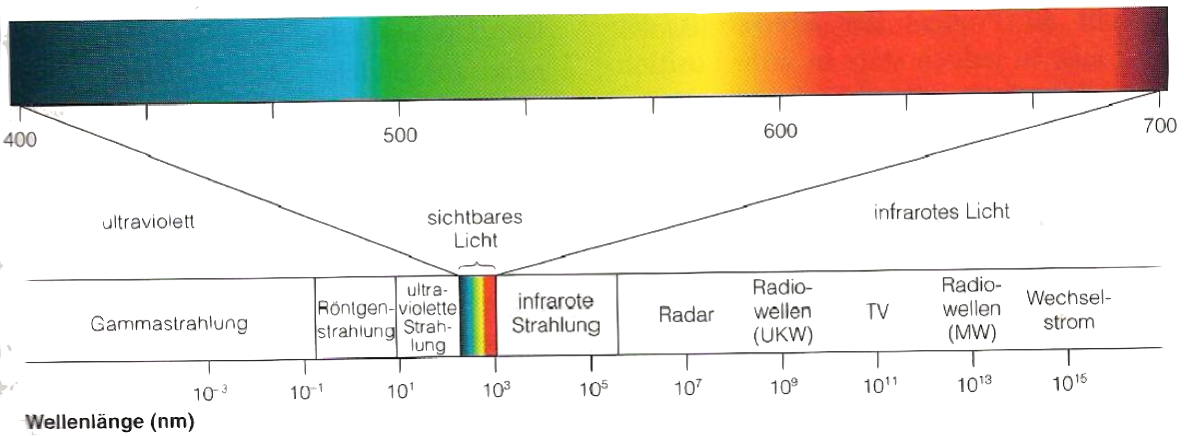
\includegraphics[width=0.9\textwidth]{abbildungen/spektralbaender.png}
    \\
    \textit{Quelle:~\cite[][\pagef 7]{ditzinger.2013}}
    \\
\end{figure}

\begin{figure}[H]
    \caption {RGB vs. 16-Band Bild}
    \label{fig:RGB_vs_16_Band}
    %\includegraphics[width=0.9\textwidth]{}
    \textcolor{red}{\textit{Hier muss noch ein Beispielbild rein...vermutlich aus unserem Datensatz}}
    \\
\end{figure}

\begin{figure}[H]
    \caption {Vergleich multispektraler und hyperspektraler Bildaufnahmen}\label{fig:multispectral_hyperspectral}
    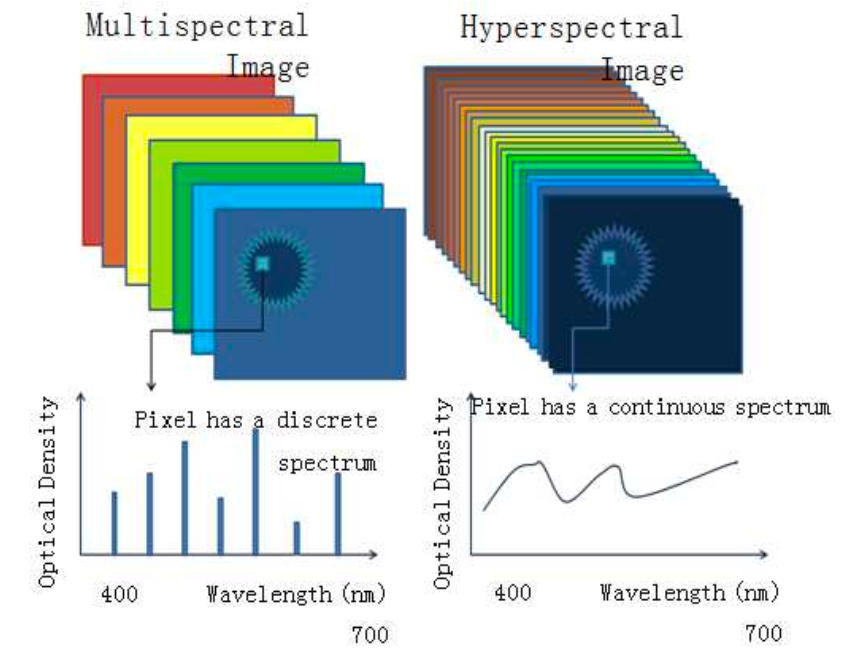
\includegraphics[width=0.9\textwidth]{abbildungen/multispectral_hyperspectral.png}
    \\
    \textit{Quelle:~\cite[][\pagef 2]{ibraheem.2015}}
    \\
\end{figure}

\begin{figure}[H]
    \caption {(a) Datenwürfel eines multispektralen Bildes, (b) Spektrum des Pixels \(P(i,j)\)}
    \label{fig:datacube_multispectral}
    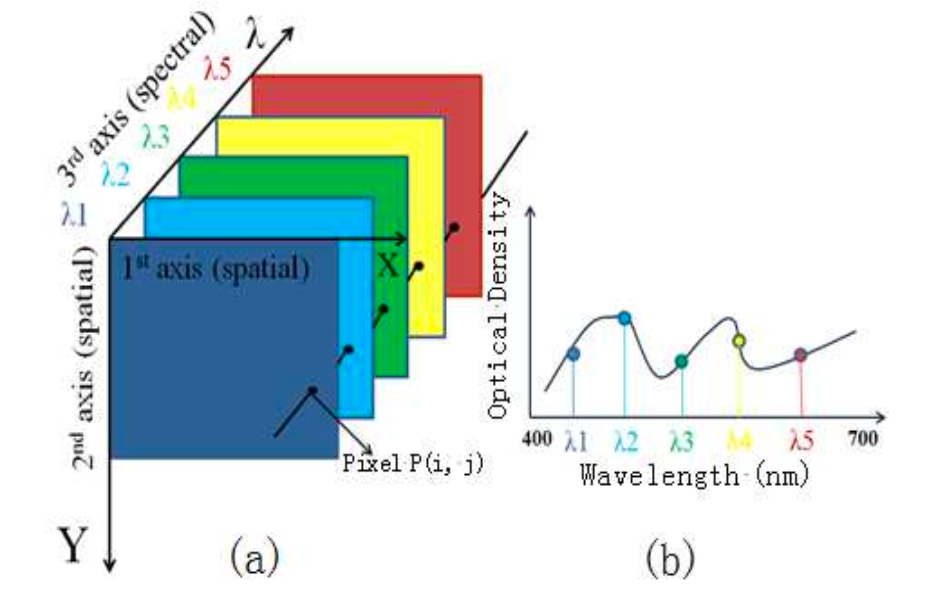
\includegraphics[width=0.9\textwidth]{abbildungen/datacube_spectral.png}
    \\
    \textit{Quelle:~\cite[][\pagef 3]{ibraheem.2015}}
    \\
\end{figure}

Die Informationen werden zeilenweise oder bandweise gespeichert.~\footcite[\vglf][\pagef 2]{upadhyay.2012}
Bei dem Zeilenweisen speichern der Bilder wird ein \(M*N\)-Bild mit \(K\)-Bändern enthält die Bilddatei \(M*K\) Zeilen
und \(N\) Spalten.
Die ersten \(K\) Zeilen der Bilddatei entsprechen dabei der ersten Pixelreihe der Aufnahme, die nächsten \(K\) Zeilen
der zweiten Pixelreihe, usw.
Bei der bandweisen Speicherung der Bilder werden die gesamten Bildinformationen je Band nacheinander gespeichert.
Es wird also jeweils eine \(M*N\) für das erste Band untereinander geschrieben, dann die \(M*N\)-Matrix für das zweite
Band, bis zum \(K\)-ten Band.

Gespeichert werden die Dateien häufig in Formaten die *.mat oder *.tif.
Bei diesen Formaten ist die Möglichkeit gegeben zusätzlich zu den Bildinformationen georgrafische Informationen wie
beispielsweise Lagedaten in Form von Koordinaten zu speichern.

\subsection{Neuronale Netzwerkarchitekturen zu Segmentierung von Satellitenbildern}

Für die maschinelle Verarbeitung von Bildern kommen häufig neuronale Netzwerkstrukturen zum Einsatz, da mit solchen in
der Vergangenheit bahnbrechende Ergebnisse auf diesem Gebiet erzielt werden konnte.~\footcite[\vglf][\pagef 1]{pritt.2020}
Die spezielle Art der Netzwerkarchitektur für solche Anwendungsgebiete sind die \ac{CNN}s.
Die Idee bei \ac{CNN}s ist es, einen oder meist mehrere rechteckige \glqq{Filter}\grqq über ein Bild schieben, was im
mathematischen Sinne einer Faltung bzw\. einer Convolution entspricht.
Ziel ist es die Gewichte der Filter so optimal zu trainieren, dass jeder Filter jeweils ein bestimmtes Merkmal eines Bildes
erkennen kann.
Je mehr Filter das neuronale Netzwerk also hat, desto mehr Merkmale kann es extrahieren und damit komplexere Muster lernen.
Der Filter wir wie oben bereits erwähnt von zu Gewichten repräsentiert, die zu trainieren sind.
Um die Rechenanforderungen zu reduzieren, wird die Größe des Filters im Laufe eines Netzwerks in der Regel kleiner,
während ihre Anzahl jedoch steigt, sodass Merkamale auf granularerer Ebene gelernt werden können.

Der ursprüngliche Zweck der \ac{CNN}-Architektur ist es einem Bild eine Klasse zuzuordnen.
Wenn Bilder mehrere Klassen enthalten, muss es zusätzlich ermöglicht werden die Größe und Lokalisierung der jeweiligen
Klassen innerhalb des Bildes zu erhalten.
Gleichzeitig muss das Netzwerk tief genug sein, um die einzelnen Klassen zu \glqq{lernen}\grqq, damit es zwischen den
Klassen unterscheiden kann.
Es kann also nicht die reine downsampling Architektur verwendet werden, wie sie es im klassischenen \ac{CNN} der Fall ist,
sondern die Informationen an welcher Stelle welche Objektklasse lokalisiert sind, müssen ebenfalls gegeben sein.
Das soeben geschilderte Problem wird durch die Idee des \ac{FCN} weitestgehend gelöst.
Während bei einem reinen \ac{CNN} die erste Schicht der Größe des Bildes entsprechen muss, da es fest mit dem
Eingabebild verbunden ist, wird bei einem \ac{FCN} das Modell ab der ersten Schicht bereits faltbar gemacht, sodass das
Modell auch gleichzeitig unabhängig von der Größe der Inputdaten ist und damit mehr Flexibilität gewährleistet.
Des Weiteren werden durch eine vollständig verbundene Schicht globale Bildinformationen verarbeitet, was sich generell
für eine Klassifizierungsaufgabe gut eignet.
Wenn es jedoch darum geht das Bild zu segmentieren sind die kleineren Faltungsschichten, die von vorn herein über das
Bild gleiten können mehr von Vorteil.
Zusammenfassend werden bei \ac{FCN}s also die voll verknüpften Schichten der \ac{CNN}s durch Faltungsschichten ersetzt.
Abbildung~\ref{fig:CNN_FCN} verdeutlicht die Funktionsweise eines \ac{CNN}, welches ein reines Katzenbild der Klasse
\glqq{Cat}\grqq zuordnet, während das \ac{FCN} dazu in der Lage die Klasse \glqq{Cat}\grqq in einem Bild mit mehreren
Klassen zu lokalisieren.
Ebenfalls ist in der Abbilung~\ref{fig:CNN_FCN} ersichtlich, dass die Auflösung der Heatmap nicht der des Eingabebildes
entspricht.
Der nächste Schritt ist demnach die grobe Merkamalszuordnung möglichst in die Ursprungsauflösung zurückzuübersetzen.
Dieser Schritt ist in der Literatur oft als \glqq{learned upsampling}\grqq bezeichnet.
Nachdem beim downsampling die Größe der Schichten immer kleiner geworden sind, um eine gewisse Detailtiefe beim Lernen
zu trainieren, ist das Vorgehen beim upsamling genau andersherum, um die Merkmalskarte auf die Ursprungsgröße des
Ausgangsbildes zu bringen.
Während beim downsampling die Filter über die Eingabedaten gleiten und Punktprodukte an jeder Position berechnen und
jeweils einen Ausgabewert weiterleiten, wird jeder Filterwert beim upsampling mit einem Eingabepixel multipliziert, über
dem der Filter positioniert ist.
Die Ergebnisse werden anschließend auf die Ausgabe-Merkmalskarte projiziert.
Filterprojetionen, die sich in der Ausgabe überschneiden werden in der regel addiert.
Abbildung~\ref{fig:upsampling} veranschaulicht die Vorgehensweise beim upsampling.
Sowohl im downsampling als auch im upsampling werden also die Filter vom neuronalen Netz trainiert.
Im Ergebnis wird also die grobe Ausgabe wieder in Pixel übersetzt.
Die Ergebnisse dabei sind jedoch ungenau und nicht trennscharf, da nur das Hinzufügen einer Upsamplingschicht allein
den großen Schritt von der Detailtiefe des Downsamplings hin zum Ausgangsformat nicht bewältigen kann.
Die Trennschärfe wird durch die sogenannte \glqq{Skip-Layer-Fusion}\grqq gelöst.
Hier werden durch Skip-Verbindungen, die eine Fusion zwischen nicht benachbarten Schichten darstellen, die Informationen
genutzt, um den räumlichen Kontext, der beim detailreichen Lernen einzelner Klassen verloren geht, mehr zu
berücksichtigen bzw\. zu übertragen
Dadurch soll das Spannungsverhältnis zwischen Detailtiefe und Lokalisierung versucht werden zu lösen.
In der Abbildung~\ref{fig:skiplayer} wird das gesamte Vorgehen einmal veranschaulicht.
Hier ist das downsampling vom Ausgangsbild bis zur letzten Faltunsschicht, die nur noch eine Dimension hat dargestellt.
Der letzte Schritt ist das upsampling, welches in der Abbildung in der obersten Reihe zu aller erst ohne Skip-Layer
Fusion dargestellt ist.
Dort ist zu erkennen, dass die Projektion der Merkmalskarte grob funktioniert.
In der zweiten Zeile werden die informationen aus der vorangehenden pool4 Schicht mit berücksichtigt, welches im Ergebnis
einen höheren Detailierungsgrad aufweist.
In der dritten Zeile werden die pool3 und die pool4 Schicht berücksichtigt, welche die Segementierungskarte noch genauer
machen.



% \begin{figure}[H]
%     \caption {\ac{CNN} und \ac{FCN} im Vergleich}
%     \label{fig:CNN_FCN}
%     %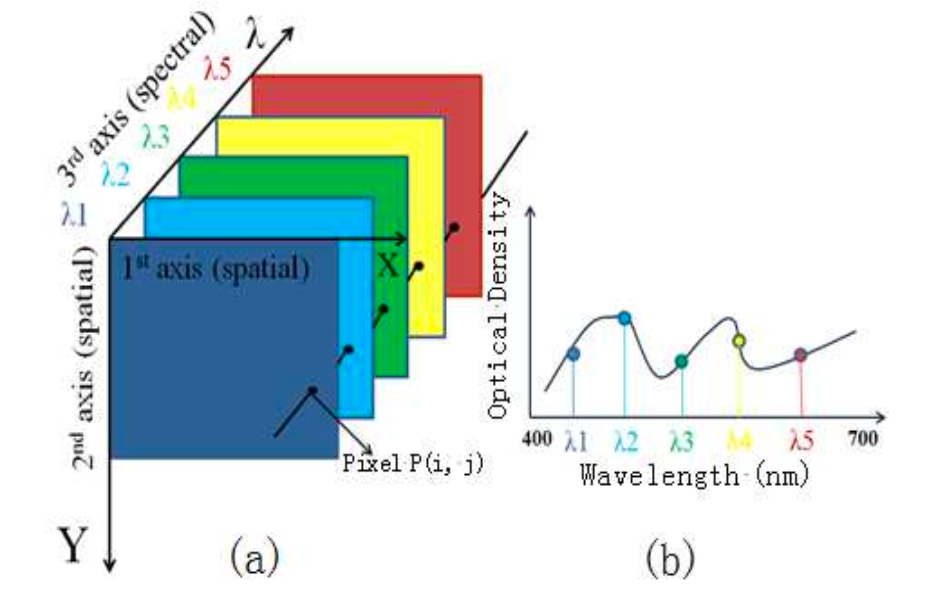
\includegraphics[width=0.9\textwidth]{abbildungen/datacube_spectral.png}
%     \\
%     \textit{\textcolor{red}{Hier muss noch das CNN und FCN rein}}
%     \\
% \end{figure}

% \begin{figure}[H]
%     \caption {Learnable Upsampling}
%     \label{fig:upsampling}
%     %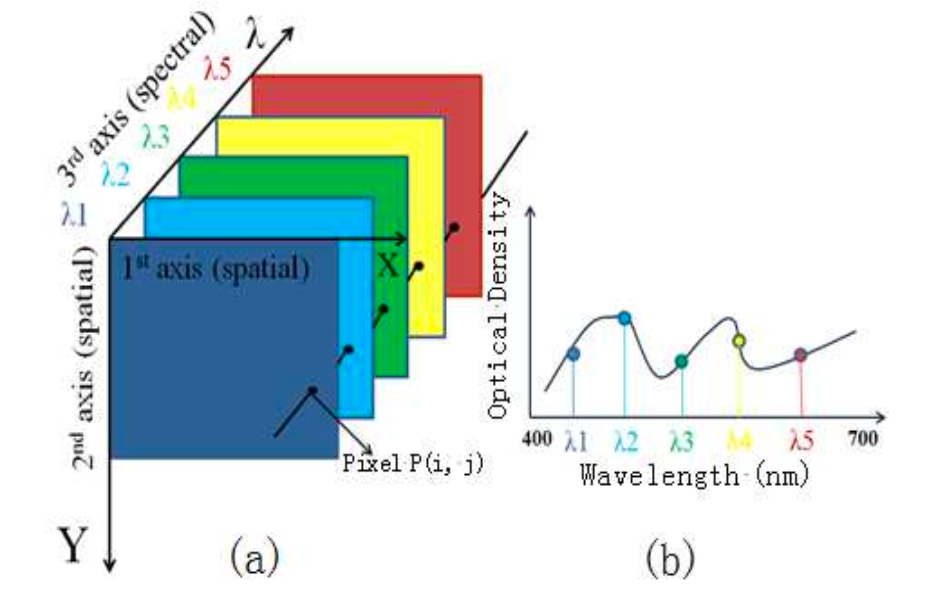
\includegraphics[width=0.9\textwidth]{abbildungen/datacube_spectral.png}
%     \\
%     \textit{\textcolor{red}{Hier muss noch das upsampling rein}}
%     \\
% \end{figure}

% \begin{figure}[H]
%     \caption {Skip Layer Fusion}
%     \label{fig:skiplayer}
%     %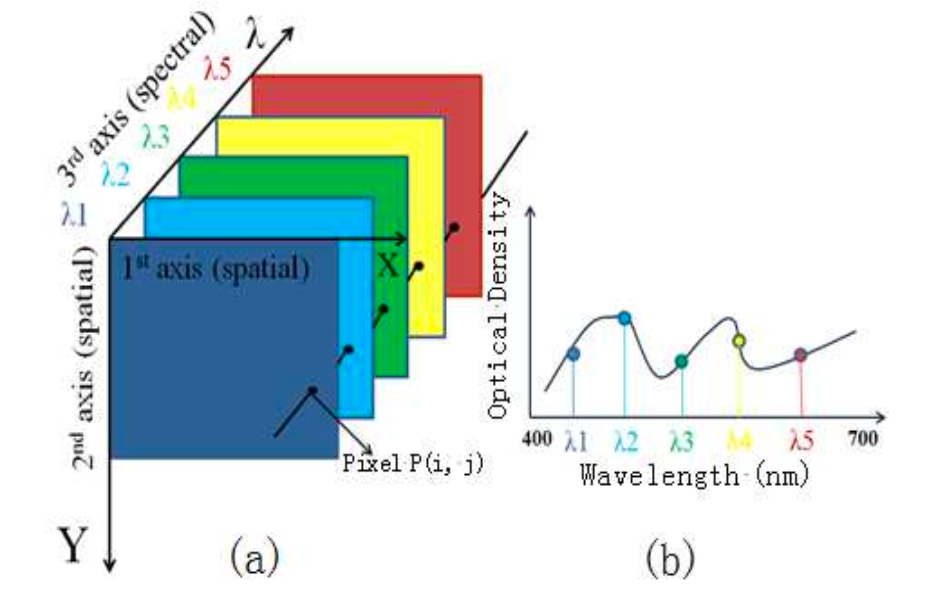
\includegraphics[width=0.9\textwidth]{abbildungen/datacube_spectral.png}
%     \\
%     \textit{\textcolor{red}{Hier muss noch die skip-Layer fusion rein}}
%     \\
% \end{figure}

Eine Weiterentwicklung des \ac{FCN}s ist das U-Net.
Dieses Modell soll die oftmals kritisierte Ungenauigkeit der \ac{FCN}s an den Segmentierungsgrenzen beheben bzw\.
optimieren.
Die Architektur der U-Net sieht aus wie der Buchstabe \glqq{U}\grqq und ist im Folgenden exemplatisch dargestellt.

\begin{figure}[H]
    \caption {U-Net}
    \label{fig:uNet}
    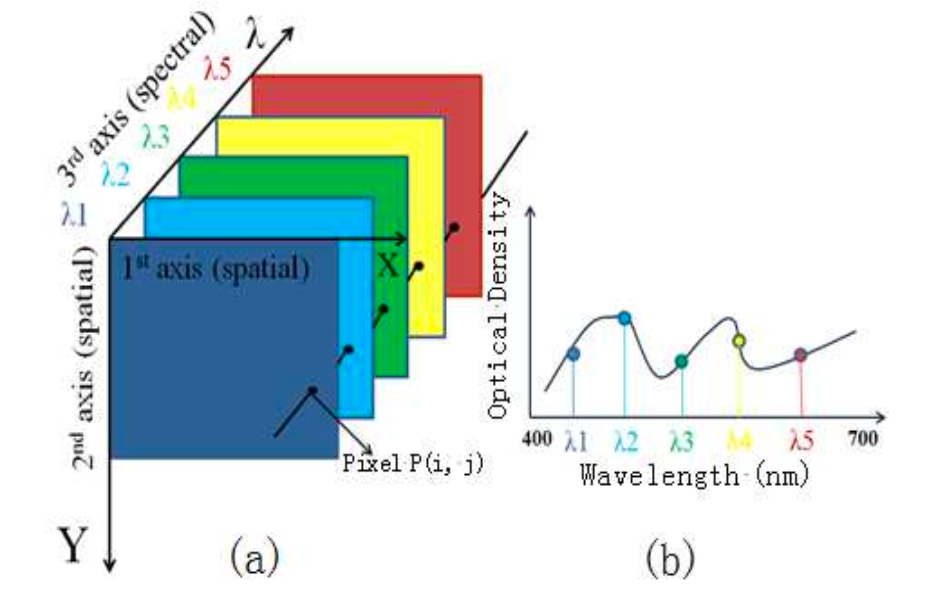
\includegraphics[width=0.9\textwidth]{abbildungen/datacube_spectral.png}
    \\
    \textit{\textcolor{red}{Hier muss noch das U-Net rein}}
    \\
\end{figure}


\subsection{Jaccard Score}
%\subsection{Vorgehen/Methodik}
%\subsubsection{IBM Prozess|CRISP mit HOT OSM Business Case}